% neighbor_diagram_v1.tex -- "Geometry" version of the diagram for eq:total-gauss.
% Single column: the bounding box is 246 pt wide (the revtex \linewidth), so
% \includegraphics[width=\linewidth] prints every size 1:1.
%
% (a) the point r, a neighbor r + d, the vector d and its angle theta_d with the x axis, the
%     neighbor's rod (headless) and its angle theta_nb with the x axis, and the angle
%     theta_nb - theta_d between the rod and the line through r and r + d (dashed beyond
%     the neighbor).
% (b) the same neighbor with its rod along d: S cos 2(theta_nb - theta_d) = +S; the rod's
%     axis (dotted) passes through r.
% (c) the same neighbor with its rod across d: -S; the rod's axis passes beside r.
% Build with ./run.sh.
\documentclass[tikz,border=0pt]{standalone}
% neighbor_preamble.tex -- shared by neighbor_diagram_v1/v2/v3.tex.
% Notation as in manuscript/definitions.tex: \r = \mathbf{r}, \bs = \boldsymbol,
% \elln = \ell_{\rm n}, \micron = \upmu\mathrm{m}. The body font is Computer Modern, as in
% revtex (no font package), and standalone sets 10 pt, so \small = 9 pt and
% \footnotesize = 8 pt print at those sizes when the pdf is included at its natural width.
\usepackage{amsmath,amssymb,upgreek}
\usepackage{xcolor}
\usepackage{tikz}
\usetikzlibrary{arrows.meta,calc}
\newcommand{\bs}{\boldsymbol}
\renewcommand{\r}{\mathbf{r}}
\newcommand{\elln}{\ell_{\rm n}}
\newcommand{\micron}{\upmu\mathrm{m}}
% the two sign colors of fig:aimed-rods (aimed_rods_exact.wls): the ends of Mathematica's
% TemperatureMap, cmap[0.97] (raises the variance) and cmap[0.03] (lowers it)
\definecolor{plusS}{rgb}{0.832,0.248,0.178}
\definecolor{minusS}{rgb}{0.226,0.355,0.936}
% the curve color of fig:omega-weight (omega_weight.wls)
\definecolor{curve}{rgb}{0.20,0.40,0.70}
\tikzset{
  >={Stealth[length=4.5pt,width=3.6pt]},
  rod/.style={line width=2.2pt, line cap=round},
  ref/.style={gray!75, line width=0.4pt},
  ang/.style={line width=0.5pt},
  pt/.style={fill=white, draw=black, line width=0.8pt},
  dvec/.style={->, line width=0.7pt},
  panel/.style={font=\small\bfseries},
}
% the point r: white disk with a black ring, as in fig:aimed-rods
\newcommand{\pointr}[1]{\filldraw[pt] (#1) circle (2.3pt);}
% the center of a neighbor rod
\newcommand{\nbdot}[1]{\fill (#1) circle (1.3pt);}

\begin{document}
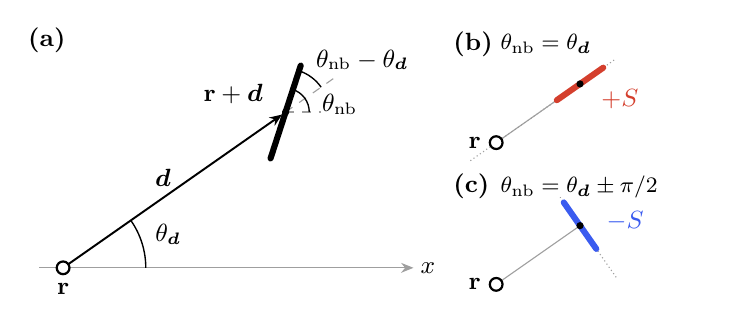
\begin{tikzpicture}[font=\small]
  \useasboundingbox (-0.45,-0.50) rectangle ++(246pt,3.55);
  % ------------------------------------------------------------- (a) geometry
  \def\thd{35}\def\thn{72}\def\L{3.45}\def\hr{0.62}
  \node[panel, anchor=north west, inner sep=0pt] at (-0.45,3.05) {(a)};
  \coordinate (r) at (0,0);
  \coordinate (n) at (\thd:\L);
  % x axis through r, and its parallel through the neighbor
  \draw[ref, ->] (-0.3,0) -- (4.45,0) node[right=-1pt, text=black] {$x$};
  \draw[ref, dashed] (n) -- ++(0.45,0);
  % the line through r and r + d, continued beyond the neighbor
  \draw[ref, dashed] (n) -- ++(\thd:0.74);
  % theta_d at r, from the x axis to d
  \draw[ang] (1.05,0) arc[start angle=0, end angle=\thd, radius=1.05];
  \node at (\thd/2:1.40) {$\theta_{\bs d}$};
  % theta_nb at the neighbor, from the x axis to the rod
  \draw[ang] ($(n)+(0.30,0)$) arc[start angle=0, end angle=\thn, radius=0.30];
  \node[anchor=west, inner sep=1pt] at ($(n)+(0.42,0.10)$) {$\theta_\text{nb}$};
  % theta_nb - theta_d at the neighbor, from the line to r to the rod
  \draw[ang] ($(n)+(\thd:0.55)$) arc[start angle=\thd, end angle=\thn, radius=0.55];
  \node[anchor=south west, inner sep=1pt] at ($(n)+(55:0.60)$)
    {$\theta_\text{nb}-\theta_{\bs d}$};
  % the vector d and the rod
  \draw[dvec, shorten >=1.6pt] (r) -- (n)
    node[pos=0.5, above left=-1pt, inner sep=2pt] {$\bs d$};
  \draw[rod] ($(n)+(\thn:\hr)$) -- ($(n)+(\thn+180:\hr)$);
  \nbdot{n}
  \pointr{r}
  \node[below=2pt] at (r) {$\r$};
  \node[anchor=south east, inner sep=1pt] at ($(n)+(165:0.26)$) {$\r+\bs d$};
  % ------------------------------------------------------------- (b), (c) limiting cases
  % local frame of each: the panel letter and the condition on the top line, r at
  % (0.2,0.09), the neighbor 1.30 away along theta_d
  \def\l{1.30}\def\hs{0.36}
  \foreach \lab/\yy/\rel/\col/\sgn/\sdir/\back/\fwd/\cond in
      {(b)/1.50/0/plusS/{+S}/-40/1.70/0.55/{\theta_\text{nb}=\theta_{\bs d}},
       (c)/-0.30/90/minusS/{-S}/10/0.80/0.44/{\theta_\text{nb}=\theta_{\bs d}\pm\pi/2}}{
    \begin{scope}[shift={(5.30,\yy)}]
      \node[panel, anchor=north west, inner sep=0pt] at (-0.35,1.50) {\lab};
      \node[anchor=north west, inner sep=0pt, font=\footnotesize] at (0.25,1.47) {$\cond$};
      \coordinate (r) at (0.2,0.09);
      \coordinate (n) at ($(r)+(\thd:\l)$);
      % the line to r, and the rod's axis (dotted): through r in (b), beside it in (c)
      \draw[ref] (r) -- (n);
      \draw[ref, densely dotted] ($(n)+(\thd+\rel:-\back)$) -- ($(n)+(\thd+\rel:\fwd)$);
      \draw[rod, \col] ($(n)+(\thd+\rel:\hs)$) -- ($(n)+(\thd+\rel+180:\hs)$);
      \nbdot{n}
      \pointr{r}
      \node[left=2pt] at (r) {$\r$};
      \node[text=\col, anchor=west, inner sep=1pt] at ($(n)+(\sdir:0.30)$) {$\sgn$};
    \end{scope}}
\end{tikzpicture}
\end{document}
